\documentclass[10pt,fleqn]{article} % Derfault font size and left-justified equations
\usepackage[%
    pdftitle={Correction des SLCI : Correcteur PI},
    pdfauthor={Xavier Pessoles}]{hyperref}

\input{style/new_style}
\input{style/macros_SII}
\usepackage{multicol}
\usepackage{siunitx}
\usepackage{schemabloc}
%\usepackage{picins}
\fichetrue
%\fichefalse

\proftrue
\proffalse

\tdtrue
%\tdfalse

\courstrue
\coursfalse

\newif\ifnormal
\normaltrue
%\normalfalse

\newif\ifdifficile
\difficilefalse
%\difficiletrue

\newif\iftdifficile
\tdifficilefalse
%\tdifficiletrue

% -------------------------------------
% Déclaration des titres
% -------------------------------------

\def\classe{\textsf{PSI$\star$ -- MP}}
\def\xxnumpartie{Cycle 03}
\def\xxpartie{Concevoir la partie commande des systèmes asservis afin de valider leurs performances}


\def\xxnumchapitre{Chapitre 1 \vspace{.2cm}}
\def\xxchapitre{\hspace{.12cm} Correction des SLCI}

\def\discipline{Sciences \\Industrielles de \\ l'Ingénieur}
\def\xxtete{Sciences Industrielles de l'Ingénieur}

\def\xxposongletx{2}
\def\xxposonglettext{1.45}
\def\xxposonglety{19}%16

\def\xxonglet{\textsf{Cycle 03}}

\def\xxactivite{TD 99}
\def\xxauteur{\textsl{Xavier Pessoles}}


\def\xxtitreexo{Quille pendulaire \ifnormal $\star$ \else \fi \iftdifficile $\star\star\star$ \else \fi }
\def\xxsourceexo{\hspace{.2cm} \footnotesize{Concours Commun Mines Ponts 2014}}

\def\xxcompetences{%
\textsl{%
\textbf{Savoirs et compétences :}\\
}}

\def\xxfigures{
\includegraphics[width=.75\textwidth]{images/fig_00}
}%figues de la page de garde
\def\xxpied{%
Cycle 03 -- Concevoir la commande des SLCI\\% afin de valider leurs performances.\\
Chapitre 1 -- \xxactivite%
}


\setcounter{secnumdepth}{5}
%---------------------------------------------------------------------------


\begin{document}
%\chapterimage{png/Fond_Cin}
\input{style/new_pagegarde}
\vspace{4.5cm}
\pagestyle{fancy}
\thispagestyle{plain}


\def\columnseprulecolor{\color{ocre}}
\setlength{\columnseprule}{0.4pt} 

\ifprof
%\begin{multicols}{2}
\else
\begin{multicols}{2}
\fi


\section*{Mise en situation}
\ifprof
\else

Les actions de l'air et de l'eau permettent au voilier d'avancer mais provoquent aussi son inclinaison autour de l'axe longitudinal $\vect{z_N}$. C’est le phénomène de gîte. Pour contrebalancer ce mouvement et éviter que le voilier ne se couche sur l’eau, la quille joue le rôle de contrepoids. 


%\begin{center}
%\includegraphics[width=.8\linewidth]{images/fig_01}
%%\textit{}
%\end{center}

Une évolution récente des voiliers de course océanique a été de les doter d’une quille pendulaire. Cette quille est en liaison pivot d’axe $\left(O,\vect{z}_N \right)$ avec la coque du navire et peut être orientée d’un côté ou de l’autre du navire. Une fois l’orientation désirée obtenue, tout mouvement dans la liaison pivot est supprimé par le blocage en rotation de celle-ci. 

\begin{center}
\includegraphics[width=.6\linewidth]{images/fig_03}

\textit{Modèle volumique 3D}
\end{center}



Afin de garantir sa répétabilité, la mise en position angulaire de la quille fait l’objet d’un contrôle par une boucle d’asservissement, dont le cahier des charges est donné ci-dessous.


\begin{center}
\begin{tabular}{|p{.7\linewidth}|c|}
\hline
Exigences & Niveau \\
\hline\hline
Stabilité : & \\
C11 : Marge de gain & \SI{10}{dB} \\
C12 : Dépassement vis-à-vis d'une entrée en échelon & Aucun \\
\hline
Rapidité :  & \\
C21 : Temps de réponse à 5\, \% & \SI{4}{s} maxi  \\
C22 : Vitesse angulaire de rotation de la quille & $8\degres/\text{s}$  maxi\\
\hline
Précision & \\
 C3 : Erreur statique vis-à-vis d'une entrée en échelon & Nulle \\
\hline
\end{tabular}
\end{center}


\subsection*{Modélisation du vérin}

La quille est manoeuvrée par deux vérins hydrauliques. Chacun d’eux est piloté par une servovalve de débit. Ce composant délivre un débit $q(t)$ proportionnel à sa tension de commande $v(t)$. Lors d’une manoeuvre de quille un seul de ces vérins est moteur et alimenté en pression via sa servovalve. L’autre est laissé dans une configuration où sa tige est libre de tout mouvement. Le déplacement terminé, la quille est verrouillée en position par un système de blocage non étudié dans ce sujet qui interdit toute circulation de fluide entre vérins et servovalves. L’angle de rotation de la quille par rapport au bâti est mesuré par un capteur potentiométrique.


Lors d’un déplacement de la quille, les mouvements d’oscillation du cylindre de vérin par rapport à la coque étant de faible amplitude et s’effectuant à de faibles vitesses, on se place dans une situation où le corps de vérin est considéré comme fixe. La tige est alors considérée en mouvement de translation galiléen.
On considère également que les mouvements étudiés sont de petits mouvements autour d’une position moyenne et que l’hypothèse des conditions initiales nulles est valide. Dans ces conditions, le comportement du vérin est défini par le modèle continu ci-dessous.

\footnotesize
\begin{center}
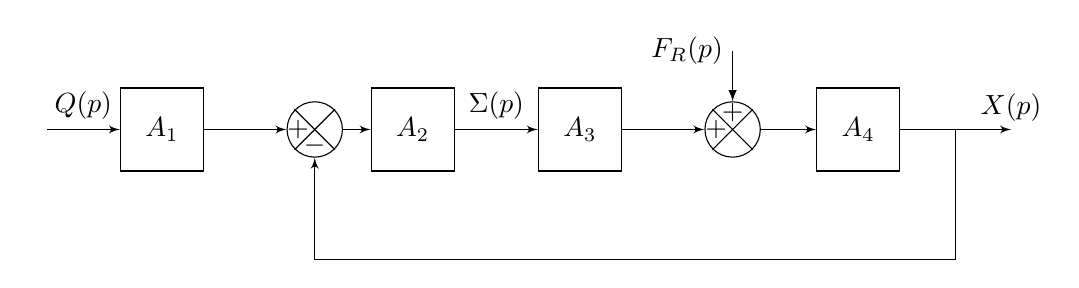
\begin{tikzpicture}
\sbEntree{E}

\sbBloc[3]{b0}{$A_1$}{E}
    \sbRelier[$Q(p)$]{E}{b0}


\sbComp{c1}{b0}
    \sbRelier{b0}{c1}

\sbBloc[1]{b1}{$A_2$}{c1}
    \sbRelier{c1}{b1}
    
\sbBloc[3]{b11}{$A_3$}{b1}
    \sbRelier[$\Sigma(p)$]{b1}{b11}


\sbSumh{c2}{b11}
    \sbRelier{b11}{c2}

\sbBloc{b2}{$A_4$}{c2}
    \sbRelier{c2}{b2}
    

\sbSortie[4]{S}{b2}
    \sbRelier{b2}{S}
    \sbNomLien[0.8]{S}{$X(p)$}
  
\sbRenvoi{b2-S}{c1}{}

\draw [latex-] (c2) --++ (0,1) node[left] {$F_R(p)$};

\end{tikzpicture}
\end{center}
\normalsize

On a : 
\begin{itemize}
\item $q(t)=S\dfrac{\dd x(t)}{ \dd t}+\dfrac{V}{2B}\dfrac{\dd \sigma(t)}{\dd t}$ (a);
\item $M\dfrac{\dd^2 x(t)}{\dd t^2} = S \sigma(t) - kx(t)-\lambda \dfrac{\dd x(t)}{\dd t} - f_R(t)$ (b).
\end{itemize}

On a :
\begin{itemize}
\item $\mathcal{L}\left(q(t)\right)=Q(p)$ : débit d’alimentation du vérin $\left[\text{m}^3\text{s}^{-1}\right]$;
\item $\mathcal{L}\left(\sigma(t)\right)=\Sigma(p)$ : différence de pression entre les deux chambres du vérin $\left[\text{Pa}\right]$;
\item $\mathcal{L}\left(x(t)\right)=X(p)$ : position de la tige du vérin $\left[\text{m}\right]$;
\item $\mathcal{L}\left(f_R(t)\right)=F_R(p)$ : composante selon l'axe de la tige du vérin de la résultante du torseur d'inter-effort de la liaison pivot entre tige et quille $\left[\text{N}\right]$.
\end{itemize}
Les constantes sont les suivantes :
\begin{itemize}
\item $S$ : section du vérin $\left[\text{m}^2\right]$;
\item $k$ : raideur mécanique du vérin $\left[N\text{m}^{-1}\right]$;
\item $V$ : volume d'huile de référence $\left[\text{m}^{3}\right]$;
\item $B$ : coefficient de compressibilité de l'huile $\left[\text{N\, m}^{-2}\right]$;
\item $M$ : masse équivalente à l'ensemble des éléments mobiles ramenés sur la tige du vérin $\left[\text{kg}\right]$;
\item $\lambda$ : coefficient de frottement visqueux$\left[\text{N m}^{-1}\text{s}\right]$.
\end{itemize} 

\subparagraph{}
\textit{Donner les expressions des fonctions de transfert $A_1$, $A_2$, $A_3$ et $A_4$ en fonction de la variable
complexe $p$ et des constantes.}


Le schéma-bloc de la figure précédente peut se mettre sous la forme suivante. 

\footnotesize
\begin{center}
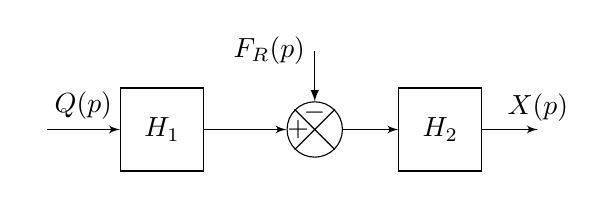
\begin{tikzpicture}
\sbEntree{E}

\sbBloc[3]{b1}{$H_1$}{E}
    \sbRelier[$Q(p)$]{E}{b1}


\sbComph{c1}{b1}
    \sbRelier{b1}{c1}
  
\sbBloc{b2}{$H_2$}{c1}
    \sbRelier{c1}{b2}

\sbSortie{S}{b2}
    \sbRelier{b2}{S}
    \sbNomLien[0.8]{S}{$X(p)$}

%\sbBloc[3]{b11}{$A_3$}{b1}
%    \sbRelier[$\Sigma(p)$]{b1}{b11}
%
%
%\sbSumh{c2}{b11}
%    \sbRelier{b11}{c2}
%
%\sbBloc{b2}{$A_4$}{c2}
%    \sbRelier{c2}{b2}
%    
%
%\sbSortie[4]{S}{b2}
%    \sbRelier{b2}{S}
%    \sbNomLien[0.8]{S}{$X(p)$}
%  
%\sbRenvoi{b2-S}{c1}{}
%
\draw [latex-] (c1) --++ (0,1) node[left] {$F_R(p)$};

\end{tikzpicture}
\end{center}
\normalsize


\subparagraph{}\textit{Donner les expressions des fonctions de transfert $H_1$
et $H_2$ en fonction de $A_1$, $A_2$, $A_3$ et $A_4$, puis de la variable $p$ et
des constantes.}
\ifprof
\begin{corrige}
\end{corrige}
\else
\fi

\subparagraph{}\textit{Pour ce vérin non perturbé ($F_R=0$), donner sa fonction de transfert $X(p)/Q(p)$ en fonction de la variable $p$ et des constantes.}
\ifprof
\begin{corrige}
\end{corrige}
\else
\fi


Le schéma d’asservissement de la position angulaire de la quille représenté figure ci-dessous sera utilisé
pour la suite des questions. La perturbation représentée par $F_R(p)$ ne sera pas prise en compte.

\footnotesize
\begin{center}
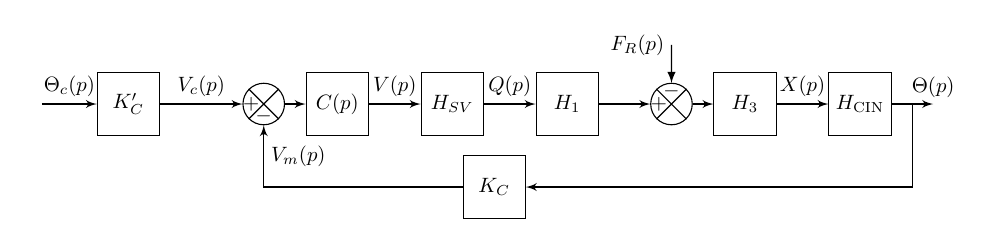
\begin{tikzpicture}[scale=0.75, every node/.style={scale=0.75}]
\sbEntree{E}

\sbBloc[3]{b0}{$K'_C$}{E}
    \sbRelier[$\Theta_c(p)$]{E}{b0}


\sbComp[5]{c1}{b0}
    \sbRelier[$V_c(p)$]{b0}{c1}

\sbBloc[1]{b1}{$C(p)$}{c1}
    \sbRelier{c1}{b1}
    
\sbBloc[2.5]{b2}{$H_{SV}$}{b1}
    \sbRelier[$V(p)$]{b1}{b2}

\sbBloc[2.5]{b3}{$H_{1}$}{b2}
    \sbRelier[$Q(p)$]{b2}{b3}
    
\sbComph[3.5]{c2}{b3}
    \sbRelier{b3}{c2}

\sbBloc[1]{b4}{$H_3$}{c2}
    \sbRelier{c2}{b4}
    
\sbBloc[2.5]{b5}{$H_{\text{CIN}}$}{b4}
    \sbRelier[$X(p)$]{b4}{b5}

\sbSortie[2]{S}{b5}
    \sbRelier{b5}{S}
    \sbNomLien[0.8]{S}{$\Theta(p)$}
  

\sbDecaleNoeudy[4]{b3}{U}
\sbBlocr{r1}{$K_C$}{U}

\sbRelieryx{b5-S}{r1}
\sbRelierxy[$V_m(p)$]{r1}{c1}

%\sbRenvoi{b2-S}{c1}{}

\draw [latex-] (c2) --++ (0,1) node[left] {$F_R(p)$};

\end{tikzpicture}
\end{center}

\normalsize


On a :
\begin{itemize}
\item $\mathcal{L}\left(\theta_c(t)\right)=\Theta_c(p)$ : consigne de position angulaire $\left[\degres\right]$;
\item $\mathcal{L}\left(\theta(t)\right)=\Theta(p)$ : position angulaire de la quille $\left[\degres\right]$;
\item $\mathcal{L}\left(v(t)\right)=V(p)$ : tension de commande de la servo valve $\left[\text{V}\right]$;
\item $\mathcal{L}\left(v_c(t)\right)=V_c(p)$ : tension image de la consigne $\left[\text{V}\right]$;
\item $\mathcal{L}\left(v_m(t)\right)=V_m(p)$ : tension image de la position $\left[\text{V}\right]$.
\end{itemize}

On a de plus :
\begin{itemize}
\item $K_c$ : gain du capteur angulaire potentiométrique $\left[\text{V}/\degres\right]$;
\item $K'_c$ : gain du bloc d'adaptation réglé tel que $K'_c=K_c=\SI{1,1}{V/\degres}$;
\item $C(p)$ : correcteur de position;
\item $H_{\text{CIN}}$ : fonction de transfert de la chaîne de transformation de mouvement dont la loi
d’entrée/sortie est supposée linéaire dans le domaine d’utilisation. $H_{\text{CIN}}=K_{\theta}$ $\left[\degres.\text{m}^{-1}\right]$;
\item $H_{\text{SV}}$ : fonction de transfert de la servo valve.
\end{itemize}

\subsection*{Modélisation de la servo valve : comportement pour une commande de grande amplitude}

La servovalve présente un fonctionnement non-linéaire provenant
d’un phénomène de saturation qui est défini par la courbe de la
figure suivante donnant les évolutions du débit $q(t)$ fourni par la
servovalve en fonction de sa tension de commande $v(t)$.
\begin{center}
\includegraphics[width=.5\linewidth]{images/fig_04}

\end{center}

Ainsi :
\begin{itemize}
\item pour $v(t) > -v_{\text{max}}$ et $v(t) < v_{\text{max}}$ : $H_{\text{sv}} = K_{\text{sv}}$ $\left[\text{m}^3 \text{s}^{-1}\text{V}^{-1}\right]$
\item pour $v(t) < -v_{\text{max}}$: $q(t) = -q_{\text{max}}$;
\item pour $v(t) > v_{\text{max}}$ : $q(t) = +q_{\text{max}}$ , $v_{\text{max}} = \SI{10}{V}$.
\end{itemize}
Le système n’est pas encore corrigé, $C(p) =1$ et on souhaite simuler
le fonctionnement où le navigateur veut déplacer la quille avec une
consigne angulaire de position de 45\degres. Cette demande est modélisée
par une consigne $\theta_c(t)$ en échelon, soit : $\theta_c(t)=\theta_0\,u(t)$ avec $\theta_0=45\degres$ et
$u(t) = 0$ pour $t < 0$ et $u(t) = 1$ pour $t > 0$. La figure suivante présente dans ces conditions les évolutions temporelles de deux grandeurs de la boucle d’asservissement, le débit sortant de la servo valve
$q(t)$ et la position angulaire de la quille $\theta(t)$.

\begin{center}
\includegraphics[width=\linewidth]{images/fig_05}
\end{center}

Sur la figure précédente, la courbe représentative de $q(t)$ présente un palier où $q(t)$ garde une valeur constante.

\subparagraph{}\textit{À l’aide de la caractéristique de la servovalve :
\begin{enumerate}
\item justifier ce palier et donner la valeur numérique de $K_{\text{SV}}$;
\item indiquer sur la figure l’intervalle de temps où le retour d’information a une influence sur la
commande du vérin et celui où il n’en a pas. Associer à chacun de ces intervalles le modèle utile :
modèle en « boucle fermée » ou en « boucle ouverte ».
\end{enumerate}}
\ifprof
\begin{corrige}
\end{corrige}
\else
\fi

\subparagraph{}\textit{Montrer, en précisant le ou les critères mis en défaut, que le cahier des charges n’est pas respecté au niveau des critères « vérifiables ».}
\ifprof
\begin{corrige}
\end{corrige}
\else
\fi

\subsection*{Comportement pour une commande de faible amplitude}
On étudie la réponse du système non corrigé ($C(p) = 1$) à une entrée échelon de 5\degres d’amplitude avec $F_R = 0$.
Le modèle de travail qui a permis de tracer les courbes de la figure précédente est :
$H_{\text{BO}}(p)=K_{\text{SV}} H_1 H_2 K_{\theta} K_C$ et $H_{\text{BO}}(p)=\dfrac{2,2}{p\left(1+0,12p + 0,04 p ^2  \right)}$.

\subparagraph{}\textit{Pour l’entrée définie ci-dessus, déterminer la valeur de la tension $v(t)$ à l’instant initial $t=0^{+}$, $v(0^{+})$.}
\ifprof
\begin{corrige}
\end{corrige}
\else
\fi


\subparagraph{}\textit{Montrer que tout au long de ce fonctionnement, la servovalve fonctionnera sans saturer.}
\ifprof
\begin{corrige}
\end{corrige}
\else
\fi



\subparagraph{}\textit{De quelle hypothèse générale d’étude des systèmes asservis ce constat participe-t-il ?}
\ifprof
\begin{corrige}
\end{corrige}
\else
\fi

Une simulation de la réponse indicielle à cet échelon de 5\degres d’amplitude a permis de tracer les courbes de la
figure suivante, obtenues pour deux valeurs du correcteur proportionnel :
\begin{itemize}
\item $C(p) = 1$ : la courbe présente des dépassements, le critère C12 n’est pas validé;
\item $C(p) = 0,44$ : tous les critères du domaine temporel sont vérifiés (C12, C21, C22, C3).
\end{itemize}

\begin{center}
\includegraphics[width=\linewidth]{images/fig_06}
\end{center}

À l’utilisation, le correcteur proportionnel réglé à 0,44 n’a pas donné satisfaction car le mouvement saccadé
de la quille dû aux fluctuations de sa vitesse de rotation générait dans certaines conditions de navigation des
perturbations compromettant la stabilité de route du navire. L’examen attentif de cette réponse indicielle
fait apparaître la persistance d’un phénomène oscillatoire dont l’origine supposée se trouve dans le
caractère résonant du vérin.


\subparagraph{}\textit{Tracer sur les figures suivantes les diagrammes d’amplitude asymptotiques de
Bode de $H_{\text{BO}}(p)$ en indiquant les valeurs numériques associées aux
points particuliers et la valeur des pentes.}
\ifprof
\begin{corrige}
\end{corrige}
\else
\fi

\begin{center}
\includegraphics[width=\linewidth]{images/fig_07}
%\textit{}
\end{center}

\subparagraph{}\textit{Déterminer par calcul la pulsation de résonance $\omega_r$ de cette fonction
de transfert.}
\ifprof
\begin{corrige}
\end{corrige}
\else
\fi


\subparagraph{}\textit{Évaluer littéralement puis numériquement à cette pulsation
$\omega_r$ la différence, notée $\Delta K$ et exprimée en dB, entre l’amplitude
de résonance et l’amplitude évaluée par le diagramme asymptotique.}
\ifprof
\begin{corrige}
\end{corrige}
\else
\fi

Pour éliminer le phénomène de résonance, on recherche l’expression de $C(p)$ permettant d’abaisser
l’amplitude de $\Delta K$ à la pulsation $\omega_r$. Le concepteur a choisi un correcteur à retard de phase de fonction de
transfert $C(p)=K_{\text{COR}} \dfrac{1+Tp}{1+bTp}$ avec $b>1$. Ce correcteur présente un extremum de la courbe de phase à la pulsation $\omega^{*}$ tel que : $\sin\left[\phi\left(\omega^{*}\right)\right]=\dfrac{1-b}{1+b}$ et $\omega^{*}=\dfrac{1}{T\sqrt{b}}$.


L’étude consiste à déterminer les valeurs de $T$ et $b$.

\subparagraph{}\textit{Tracer sur la figure suivante, les diagrammes d’amplitude et de phase (asymptotiques et allure
de la courbe réelle) de Bode de ce correcteur pour $K_{\text{COR}} =1$. Préciser les expressions littérales des
pulsations caractéristiques.}
\ifprof
\begin{corrige}
\end{corrige}
\else
\fi

\begin{center}
\includegraphics[width=\linewidth]{images/fig_08}
%\textit{}
\end{center}


\subparagraph{}\textit{Déterminer alors en fonction de $b$, l'amplitude $\left| C\left(j\omega^{*}\right)\right|_{\text{dB}}$ à la pulsation notée $\omega^{*}$. }
\ifprof
\begin{corrige}
\end{corrige}
\else
\fi

Pour $K_{\text{COR}} =1$, en faisant correspondre la pulsation de résonance $\omega_r$ de $H_{\text{BO}} =1$ à $\omega^{*}$.

\subparagraph{}\textit{Calculer $b$ pour que « l’excès » de gain $\Delta K$ soit compensé par le correcteur et calculer la valeur de $T$.}
\ifprof
\begin{corrige}
\end{corrige}
\else
\fi

\subparagraph{}\textit{Calculer le supplément de déphasage introduit par le correcteur à la pulsation $\omega^{*}$.}
\ifprof
\begin{corrige}
\end{corrige}
\else
\fi

La réponse indicielle correspondant à ce réglage (entrée échelon de 5\degres d’amplitude) est donnée sur la figure suivante. Le gain $K_{\text{COR}}$ a été déterminé de façon à satisfaire les critères C11 et C12.

\begin{center}
\includegraphics[width=\linewidth]{images/fig_09}
%\textit{}
\end{center}


\subparagraph{}\textit{Déterminer la vitesse de rotation angulaire maximale de la quille obtenue avec ce réglage du
correcteur.}
\ifprof
\begin{corrige}
\end{corrige}
\else
\fi

\subparagraph{}\textit{Validez les critères C21 et C22 en laissant vos constructions apparentes.}
\ifprof
\begin{corrige}
\end{corrige}
\else
\fi
\end{multicols}


\end{document}

\subparagraph{}\textit{}
\ifprof
\begin{corrige}
\end{corrige}
\else
\fi

\begin{center}
\includegraphics[width=\linewidth]{images/fig_04}
%\textit{}
\end{center}

